Individual accuracy and loss curves for all 6 models can be found in Appendix C. The models were prepared using the preparation code from \cite(ADD GITHUB PAGE) and uploaded to Kaggle to infer on the test set. The scores indicate the area under the ROC curve, or AUC. The private scores have been chosen due to the fact that those scores are calculated with about 80\% of the test data and therefore represent a better efficiency in the model.
\begin{table}[h]
\centering
\begin{tabular}[width=0.7\textwidth]{|c|c|c|c|c|}
\hline
\textbf{amount of dense layers} & \textbf{AUC 4 CN layers} & \textbf{AUC 3 CN layers} \\ \hline
4 & 0.8903 & 0.8954\\ \hline
3 & 0.9045 & 0.9093 \\ \hline
2 & 0.8823 & 0.9121\\ \hline
\end{tabular}
\caption{Summary of AUC Scores for each model submitted to Kaggle}
\label{AUC table}
\end{table}

\begin{figure}
    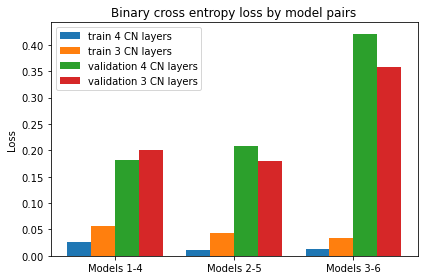
\includegraphics[width=0.4\textwidth]{images/loss.png}
    \caption{Loss per model during training and validation}
    \label{Lossgraph}
 \end{figure}
 \begin{figure}
    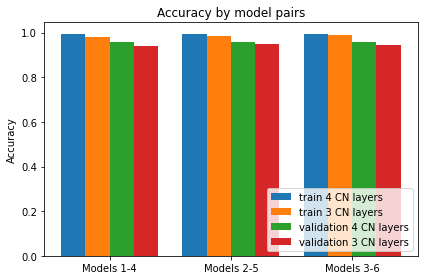
\includegraphics[width=0.4\textwidth]{images/ac.png}
    \caption{Accuracy per model during training and validation}
    \label{ACgraph}
\end{figure}

The performance during machine learning has been summarized in graph \ref{Lossgraph} and \ref{ACgraph}, and use the data found in \ref{ACtable}. These show a comparison of the models with 4 CN layers and the models with 3 CN layers in decreasing order of amount of dense layers.